\documentclass[12pt]{extarticle}
\usepackage[utf8]{inputenc}
% \usepackage{cite}
\usepackage{graphicx}
\usepackage{booktabs}
\usepackage{adjustbox}
\usepackage[letterpaper, margin=1in]{geometry}

\title{Basic Three-Sided Market Model}
\author{Block Science}
\date{March 2019}

\begin{document}

\maketitle

\begin{figure}
    \centering
    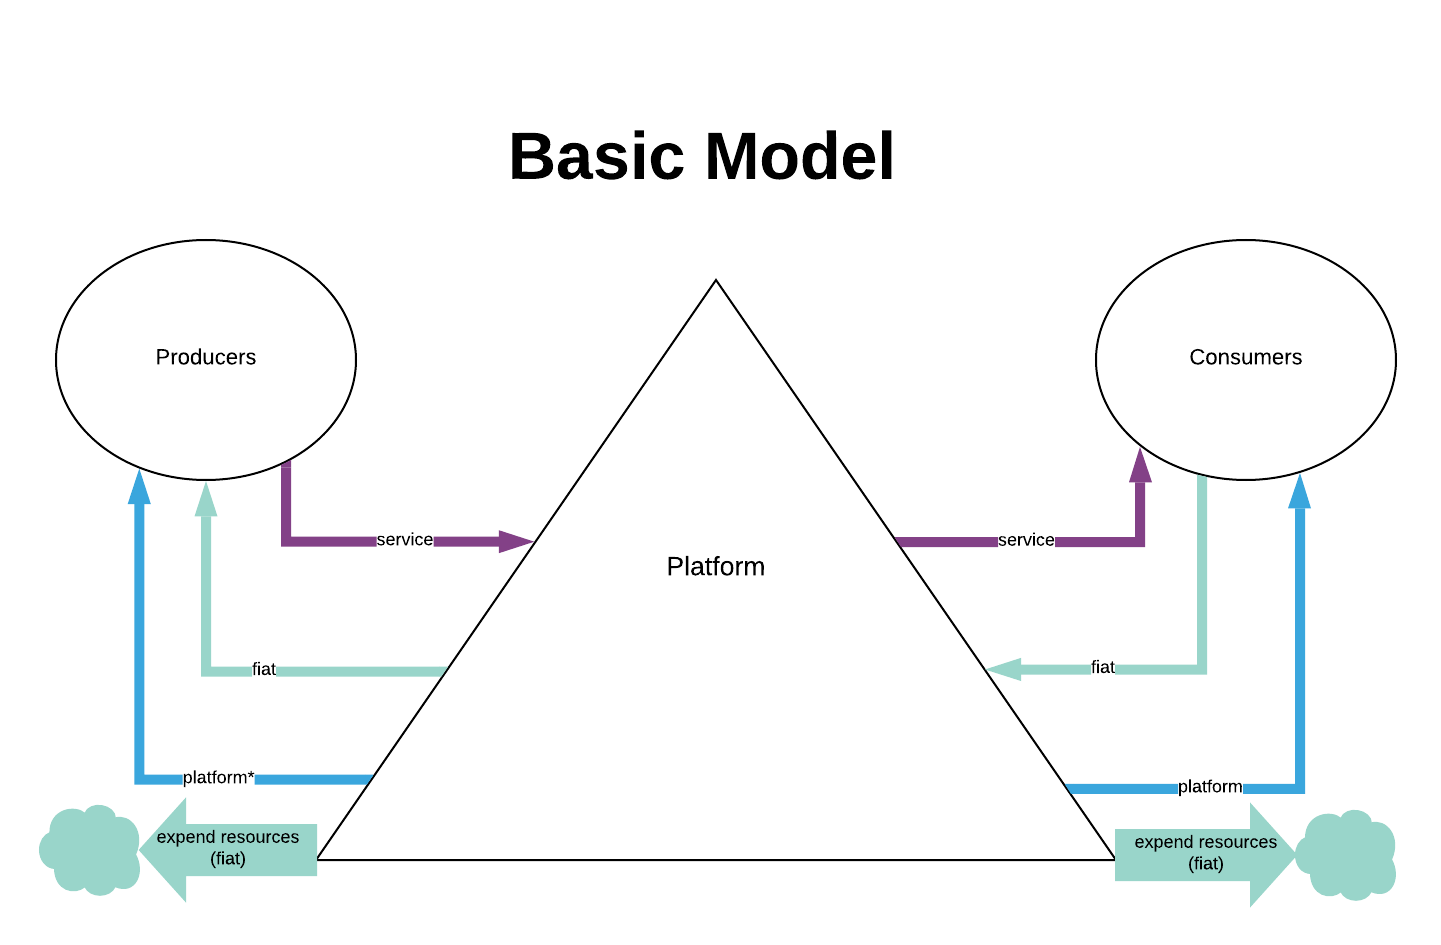
\includegraphics[width=1\textwidth]{images/3SidedMarketBasicDemo.png}
    \caption{Basic Three-Sided Market Model}
    % \label{fig:my_label}
\end{figure}

\section{Introduction}
The ‘Three-Sided Market’ model is for platform business where the product being produced enables transactions between a service provider and service consumer. The reference example for this case is a ride sharing app such as Uber. In this case drivers would be providers and riders would be consumers. The corporation Uber is the producer, and in our three-sided-market that role will be spread to a decentralized community collectively providing all of the functions required for users (providers and consumers) to have an equivalent user experience. \\

This work is part of the ongoing economic systems research at BlockScience. We would be thrilled to have you build on our work, but please cite us if you do. \\

Models presented are note predictions or final designs, merely 'what-if' explorations of complex sociotechnical systems. Contact media@block.science with interest in our methods and tools.


\section{Building a Model of a Three-Sided Market}
To construct our model, we will use our internally developed simulation tool called cadCAD. \\

cadCAD is a differential games based simulation software package for research, validation, and Computer Aided Design of economic systems created by BlockScience. An economic system is treated as a state-based model and defined through a set of endogenous and exogenous state variables which are updated through mechanisms and environmental processes, respectively. Behavioral models, which may be deterministic or stochastic, provide the evolution of the system within the action space of the mechanisms. Mathematical formulations of these economic games treat agent utility as derived from the state rather than direct from an action, creating a rich, dynamic modeling framework. Simulations may be run with a range of initial conditions and parameters for states, behaviors, mechanisms, and environmental processes to understand and visualize network behavior under various conditions. Support for A/B testing policies, Monte Carlo analysis, and other common numerical methods is provided. \\ 

What that essentially means is cadCAD allows us to use code to help solidify our conceptualized ideas and run them to see if the outcome meets our expectations. We can then iteratively refine our work until we have constructed a model that closely reflects reality at the start of the model, and see how it evolves. We can then use these results to inform business decisions.

\section{Build individual components}
Before we will create a holistic model that takes into account all of the individual components and how they interact in our `dynamic system', we will construct below individual components and explain their structure.

\subsection{Transaction Growth Rate}
Below we construct a stochastic (random) s-shaped growth curve to represent the transaction volume of the ecosystem. See figure \ref{fig:components}

\subsection{Product Cost}
Create a random process to represent the growth of the cost of production, due to inflation, etc over time. See figure \ref{fig:components}
\\
\begin{figure}[h]
    \centering
    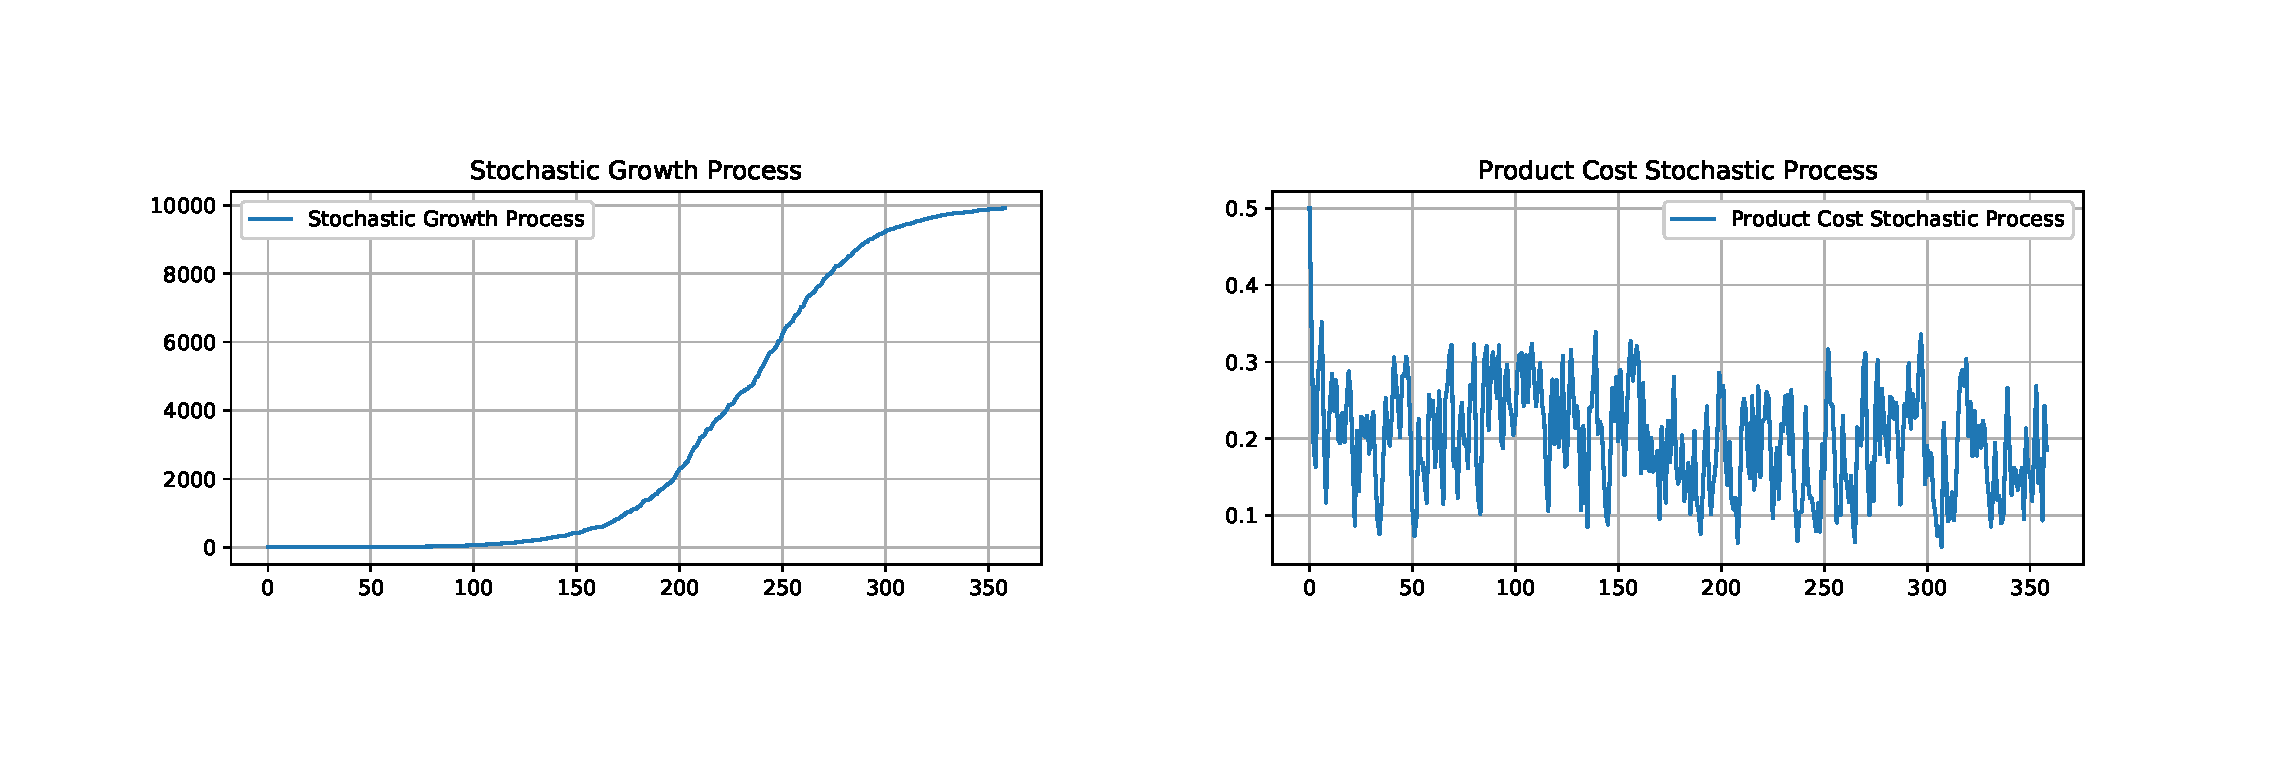
\includegraphics[width=1\textwidth]{images/components.eps}
    \caption{Components}
    \label{fig:components}
\end{figure}

\section{cadCAD Simulation}
In the background, we have finished defining a configuration file that contains the mathematical specifications and simulation commands, examples of which are shown in the previous section and run our model.
We look the results at the beginning and the ending of our model to see we started on 2019-03-01 and allowed our model to evolve until 2020-02-24. See the first five results at table \ref{table:FirstFive} and the last five at table \ref{table:LastFive}. \\ 


\begin{table}[h]
	\centering
	\begin{adjustbox}{max width=\textwidth}
	\begin{tabular}{lllllllllll}
		\toprule
		& fiat\_reserve & overhead\_cost & product\_cost & revenue & run & seed\_money & substep & time                & timestep & tx\_volume \\
		0 & 0.0           & 10000.0        & 0.3           & 0.0     & 1   & 10000.0     & 0       & 2018-01-01 00:00:00 & 0        & 10.0       \\
		1 & 0.0           & 10010.0        & 0.34          & 0.0     & 1   & 9700.0      & 1       & 2018-01-02 00:00:00 & 1        & 10.41      \\
		2 & 26.02         & 10010.0        & 0.34          & 26.02   & 1   & 9700.0      & 2       & 2018-01-02 00:00:00 & 1        & 10.41      \\
		3 & 9726.02       & 10010.0        & 0.34          & 26.02   & 1   & 9700.0      & 3       & 2018-01-02 00:00:00 & 1        & 10.41      \\
		4 & -283.98       & 10010.0        & 0.34          & 26.02   & 1   & 9700.0      & 4       & 2018-01-02 00:00:00 & 1        & 10.41  \\ \bottomrule   
	\end{tabular}
\end{adjustbox}
\caption{First five time steps of the Monte Carlo Run}
\label{table:FirstFive}
\end{table}

\begin{table}[h]
	\centering
	\begin{adjustbox}{max width=\textwidth}
	\begin{tabular}{lllllllllll}
		\toprule
		& fiat\_reserve & overhead\_cost & product\_cost & revenue    & run & seed\_money & substep & time                & timestep & tx\_volume \\
		1436 & 809467.72     & 13590.0        & 0.16          & 4722340.15 & 1   & 0.18        & 4       & 2018-12-26 00:00:00 & 359      & 9994.42    \\
		1437 & 809467.72     & 13600.0        & 0.08          & 4722340.15 & 1   & 0.17        & 1       & 2018-12-27 00:00:00 & 360      & 9994.66    \\
		1438 & 834454.36     & 13600.0        & 0.08          & 4747326.79 & 1   & 0.17        & 2       & 2018-12-27 00:00:00 & 360      & 9994.66    \\
		1439 & 834454.53     & 13600.0        & 0.08          & 4747326.79 & 1   & 0.17        & 3       & 2018-12-27 00:00:00 & 360      & 9994.66    \\
		1440 & 820854.53     & 13600.0        & 0.08          & 4747326.79 & 1   & 0.17        & 4       & 2018-12-27 00:00:00 & 360      & 9994.66 \\ \bottomrule
	\end{tabular}
\end{adjustbox}
\caption{Last five time steps of the Monte Carlo Run}
\label{table:LastFive}
\end{table}

We plotted the results of the simulation below in figure \ref{fig:results}. We can see that the Fiat Reserve initially decreased into negative territory while the company was getting started (we are assuming the model starts at day one of the company, or new business venture). Initially the company receives an injection of capital through VC seed money, although this trails off over time as the company matures. The overhead costs steadily increase through the simulation, however the product cost varies significantly, but is on downward sloping trend and the company becomes more efficient. We see that revenue starts off at 0 and takes a while to ramp up (as would be expected for a start-up, hence the initial cash flow problem). And finally, we examine the transaction volume, and as it is an exogenous (external to the system) process, it follows the same s-shaped curve we built as an individual component above. 
\newpage

\begin{figure}[h]
    \centering
    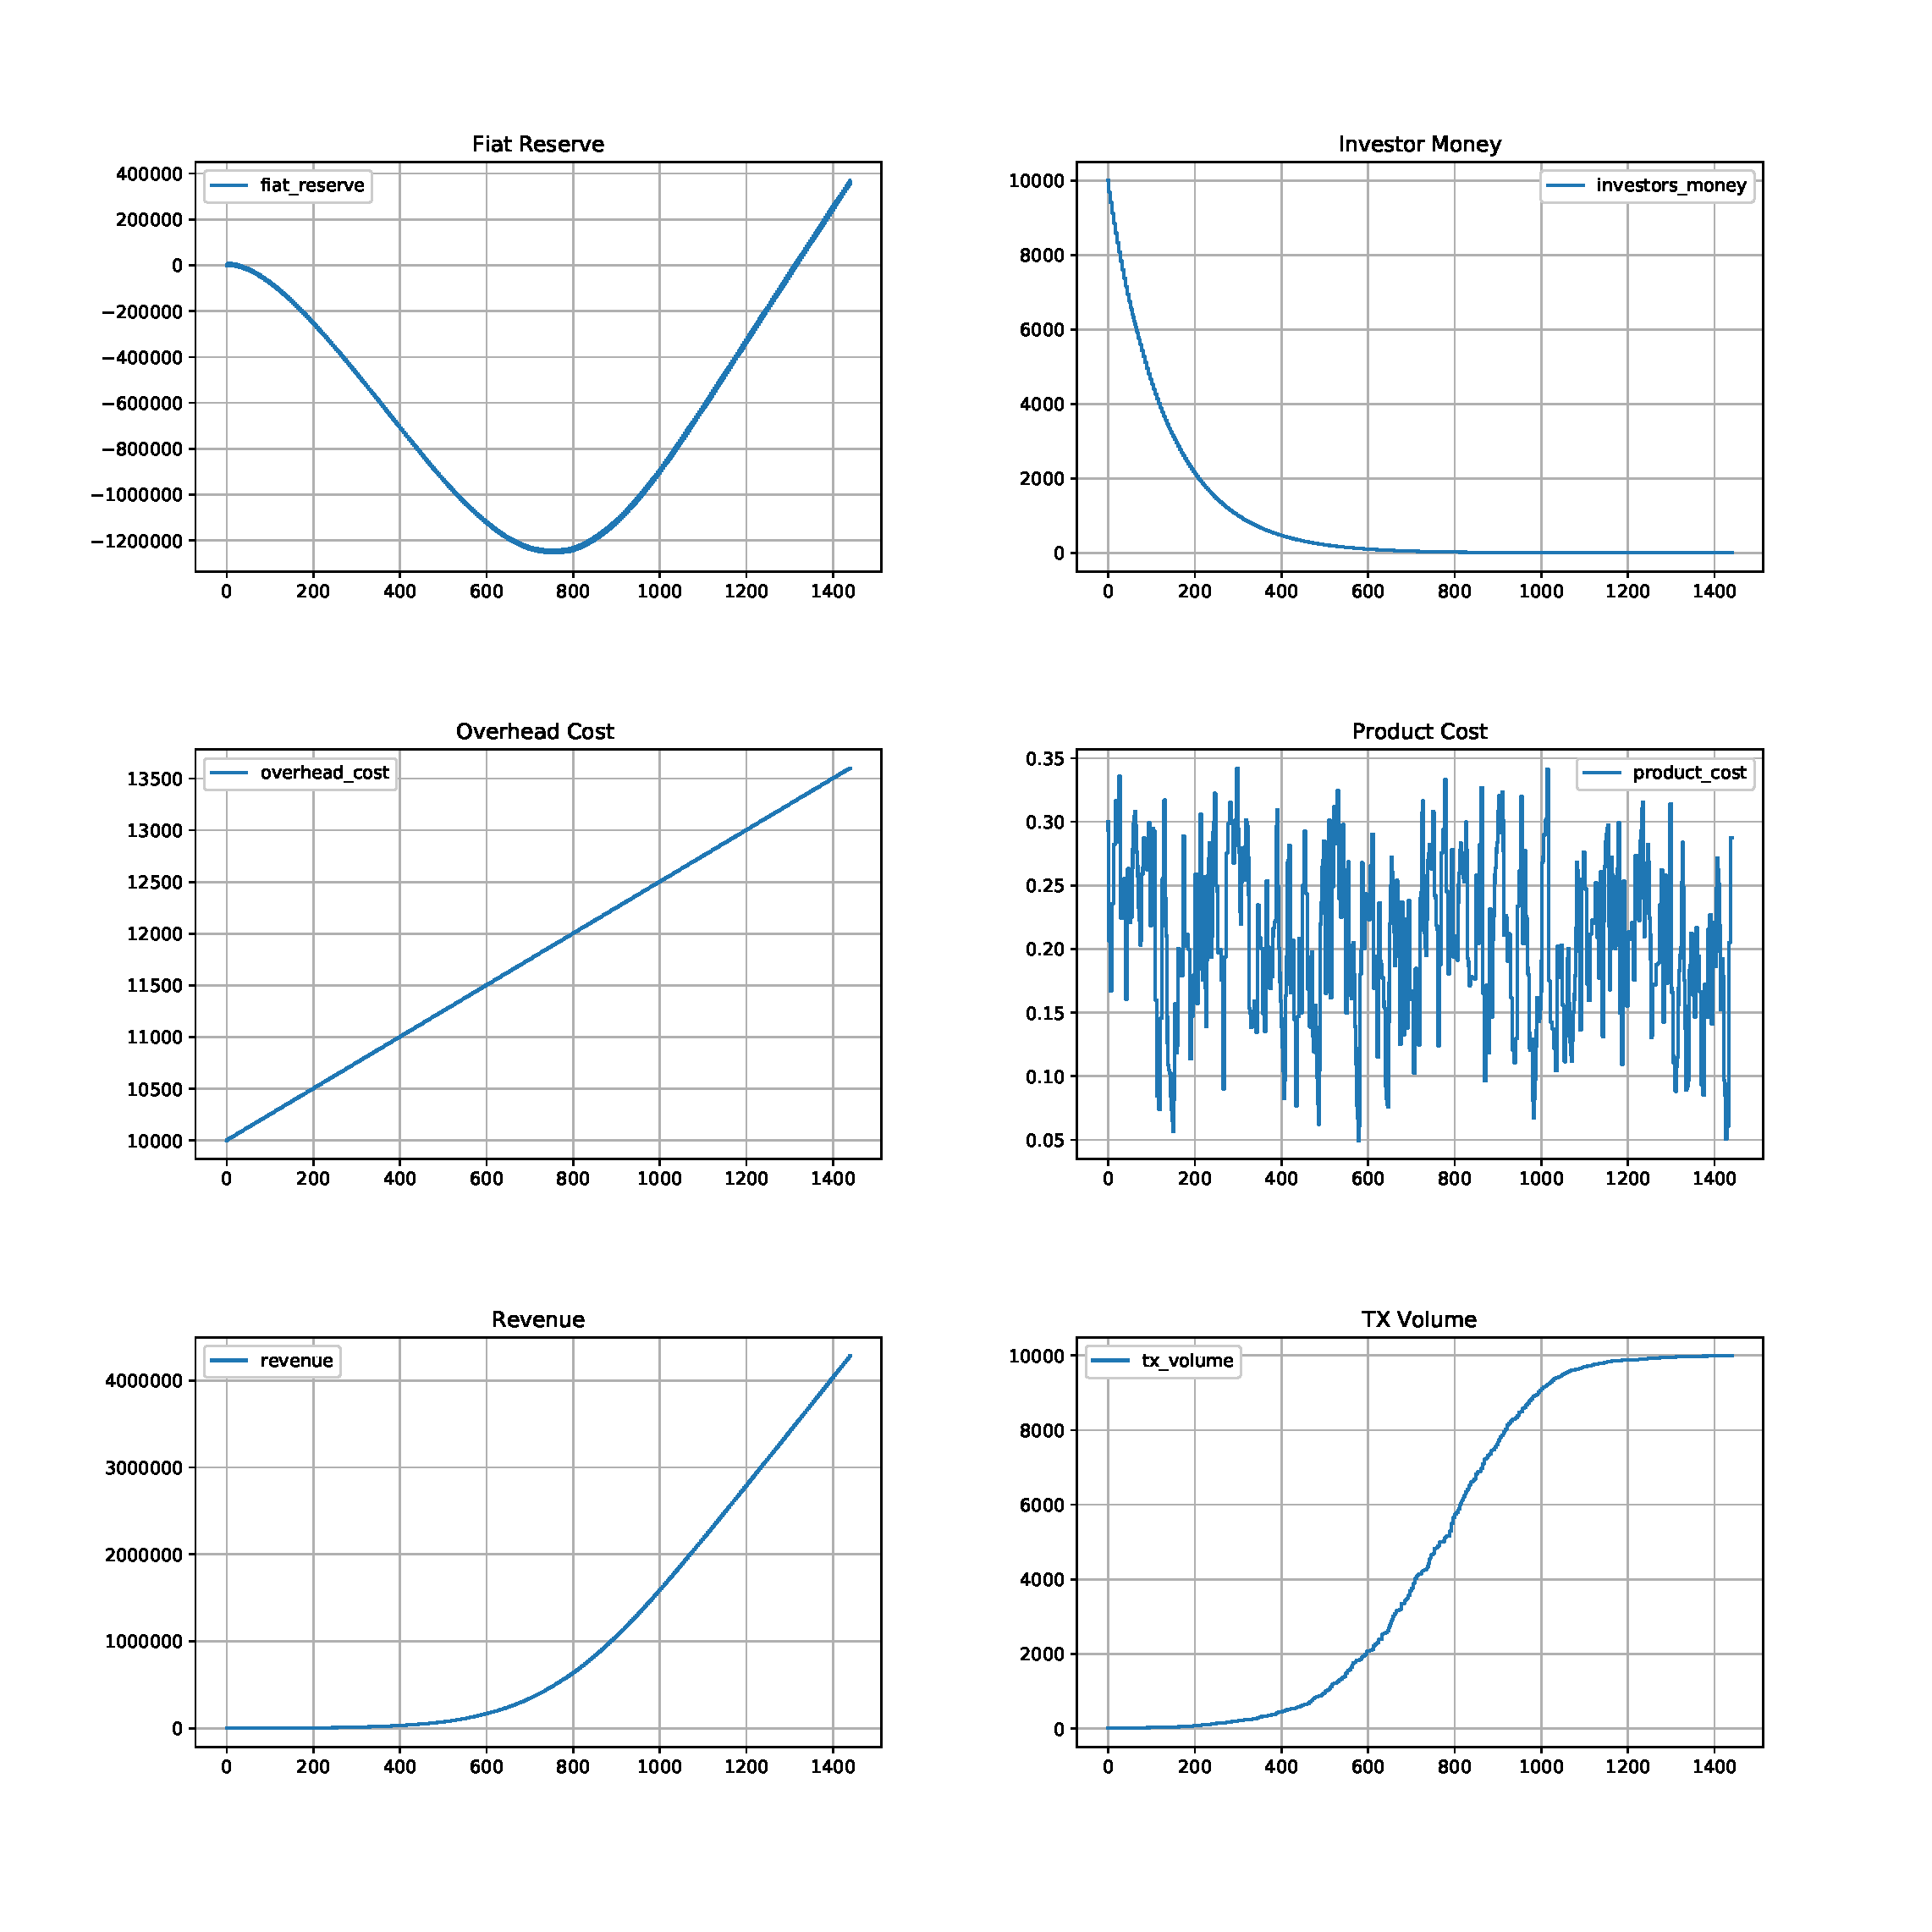
\includegraphics[width=1\textwidth]{images/Results.eps}
    \caption{Results}
    \label{fig:results}
\end{figure}


\section{Conclusion}
We have walked through a basic dynamical system ecosystem model taking in some external variables and see how the system responds to these signals and evolves. We observe that the policy and pricing incentives built into the model represent a successful business model. Now, this is an extremely simplistic model and lacks more rigorous assumptions and testing, but provides an excellent jumping off point for showing how we model dynamic complex systems. Significantly what makes our modeling approach so powerful, is we can A/B Test, or in other words, try slightly different policies and see how the system interacts and how the outputs we are concerned about respond. It is very effective mechanism for making business decisions. Our cadCAD tool and methodology allow us to represent a company's current business model adequately and future desired state and help make informed, rigorously tested decisions on how to get you from point a to point b.
\end{document}

